\section{Environment Definition}


\subsection{Cartpole}
Its observation space consists of position of the cart on the horizontal axis and its velocity and the angle of the pole and its angular velocity.
The objective of this environment is to balance the pole over 500 episodes
To balance the pole the angle needs to stay in between $\pm12^\circ$ and the cart position stay in between the bounds of $\pm2.4$
The reward system is for cartpole is very simple, it earns 1 point for each time step survived.
\cite{cartpole}

\subsection{2D Walker}
The 2d environment uses as a physics engine Pymunk \cite{pymunk}, a python implementation of Chipmunk\cite{chipmunk} 
in conjunction with pygame \cite{pygame} to render the simulation. 
%extend the decision of pygame and pymunk in this paragraph ^

To achieve walking a 2D simplified humanoid was developed in this environment, it consists of 8 joints, shoulder, hips, knees and ankle.
%check degrees of freedom
\begin{figure}[h]
    \centering
    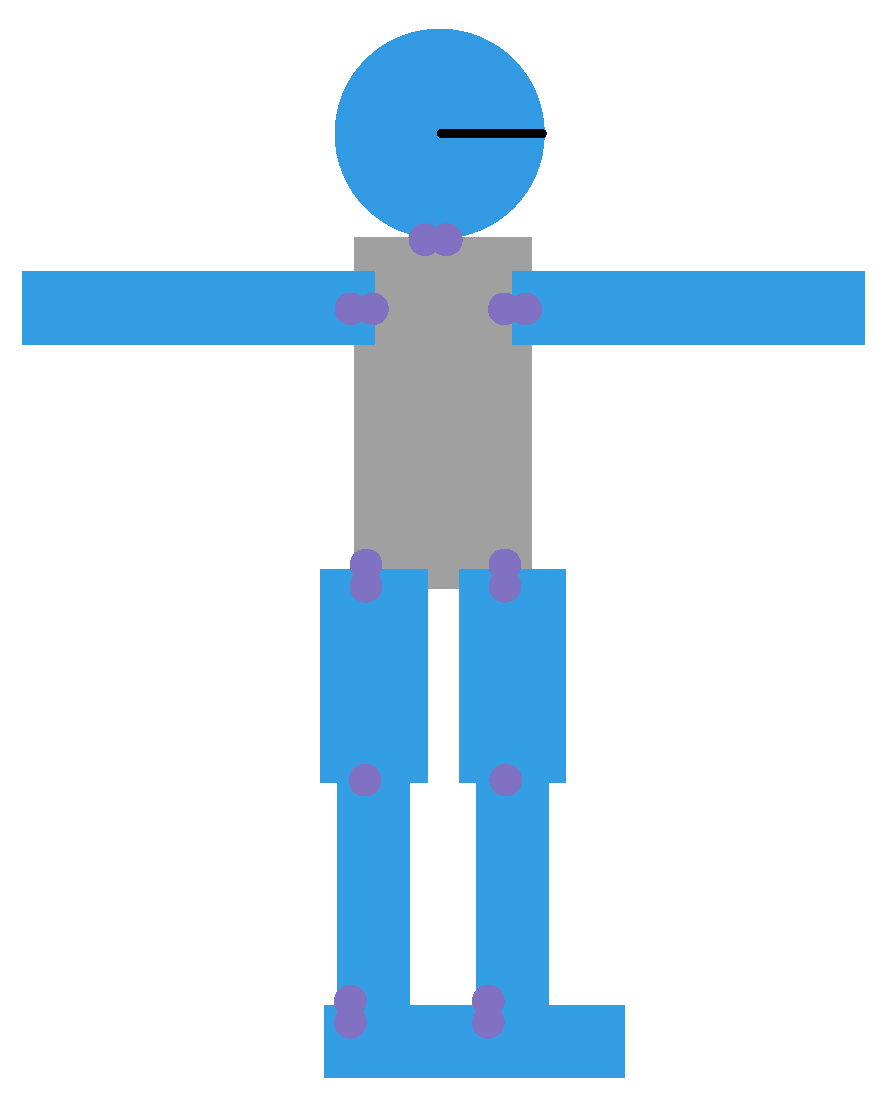
\includegraphics[scale=0.25]{humanoid-2d}
    \caption{Representation of 2D humanoid}
\end{figure}

The reward system developed for this environment:
\begin{itemize}
    \item Moves back: penalty of 200 points
    \item Stays in place: penalty of 100 points
    \item Moves forward: receives 0 points
    \item Both feet lose contact with the ground: cumulative penalty of 50 points
    \item Reaches target position: reward of 100 points
    \item Falls: penalty calculated as $\frac{1}{1-\gamma}\cdot$(highest penalty) 
\end{itemize}

\subsection{3D Walker}


\cite{ros-gym}
